\documentclass[12pt]{article}
\usepackage[utf8]{inputenc}
\usepackage{geometry}
\geometry{a4paper, top=1.25cm,bottom=1.5cm,right=1.5cm,left=1.5cm}
\usepackage{amsmath, amssymb, amstext}
\usepackage{tikz}
\usepackage{pdfpages}
\setlength\parindent{0pt}
\tikzset{myBound/.style={color=blue}}
\tikzset{myAxisLine/.style={line width=0.3mm,color=black}}
\tikzset{myLine/.style={thick,color=black}}
\usepackage{enumitem}
\usepackage{array}
\newcolumntype{M}{> {$} l < {$}}
\usepackage{mathtools}
\newcommand\Mycomb[2]{\prescript{#1\mkern-1mu}{}C_{#2 \mkern+6mu}}
\renewcommand{\baselinestretch}{1.2}
\usepackage{tkz-euclide}
\usetikzlibrary{positioning}

\usepackage{hyperref}
\hypersetup{
	colorlinks=true,
	linkcolor=blue,
	filecolor=magenta,      
	urlcolor=cyan,
}

\definecolor{minGridCol}{RGB}{130, 255, 255}
\tikzset{myMajGrid/.style={color=gridCol, line width=0.0mm}}
\tikzset{myMinGrid/.style={color=minGridCol, line width=0mm}}
\tikzset{myAxisLine/.style={line width=0.3mm,color=black}}

\usepackage{tkz-euclide}

\tikzset{myAngle/.style={thin,color=black}}
\newcommand\onelabel[6]{
	\tkzMarkAngle[myAngle,size =#1]({#2},{#3},{#4})
	\tkzLabelAngle[pos=#5 ]({#2},{#3},{#4}){\footnotesize ${#6}$}
}

\title{Binomial Theorem}
\author{Kh notes}
\date{}

%--------------------
\newcommand\LineControl[3]{

	\begin{tikzpicture}
		\draw[white, ultra thick](0,#2*0.5)--(#3,#2*0.5);
		\foreach \y in { 0,...,\fpeval{#1 -1} }{
			\draw[line width=0mm](0,-\y*#2)--(#3,-\y*#2);
	}\end{tikzpicture}
}
%--------------------


%----------------------Triangles------------------------------------------
\newcommand{\x}{0}
\newcommand{\y}{0}
\newcommand\triangleSAS[7]{
	\renewcommand{\x}{0};
	\renewcommand{\y}{0};
	\coordinate (R) at (#5,#6);
	%\filldraw[red](\x,\y) circle [radius=1pt];
	%\filldraw[](0,0) circle[radius=1pt];
	\begin{scope}[ xshift=#5cm, yshift=#6cm,rotate around={#4:(R)}, scale around={#7:(R)} ]
		%\filldraw[blue](\x,\y) circle [radius=1pt];
		\coordinate(O) at(0,0);
		\coordinate(B) at (#3,0);
		\coordinate(A) at ({#1*cos(#2)},{#1*sin(#2)});		
	\end{scope}
	
}


%----------------------Bounding Boxes------------------------------------------
\newcommand\brect[2]{
	\draw[myBound](-#1,-#2)rectangle(#1,#2);
	%backcolour
	\draw[myBound, opacity=0.1, xstep=0.5cm, ystep=0.5cm](-#1,-#2)grid(#1,#2);
	\draw[myBound](0,0)circle[radius=2pt];
}
\begin{document}
	\maketitle
	\tableofcontents
	\newpage
\section{Factorial Notation}
We define $n!$ as
$$n! = n(n-1)(n-2)...3\times 2 \times 1$$
And define $0! = 1$
\subsection{Ex 1A}
\newpage
\section{Binomial Expansions}
\def\arraystretch{2}
\setlength\tabcolsep{0.2cm}
\begin{center}
	Pascal's Triangle\vspace{1cm}\\
	\begin{tabular}{*{15}{c}}
		&&&&&&1&&1&&&&&& \\
		&&&&&1&&2&&1&&&&& \\
		&&&&1&&3&&3&&1&&&& \\
		&&&1&&4&&6&&4&&1&&& \\
		&&1&&5&&10&&10&&5&&1&& \\
		&1&&6&&15&&20&&15&&6&&1& \\
		1&& 7&&21 &&35 &&35 &&21 &&7 && 1 \\
	\end{tabular}\vspace{1cm}
\end{center}
	\begin{figure}[!h]
		\centering
	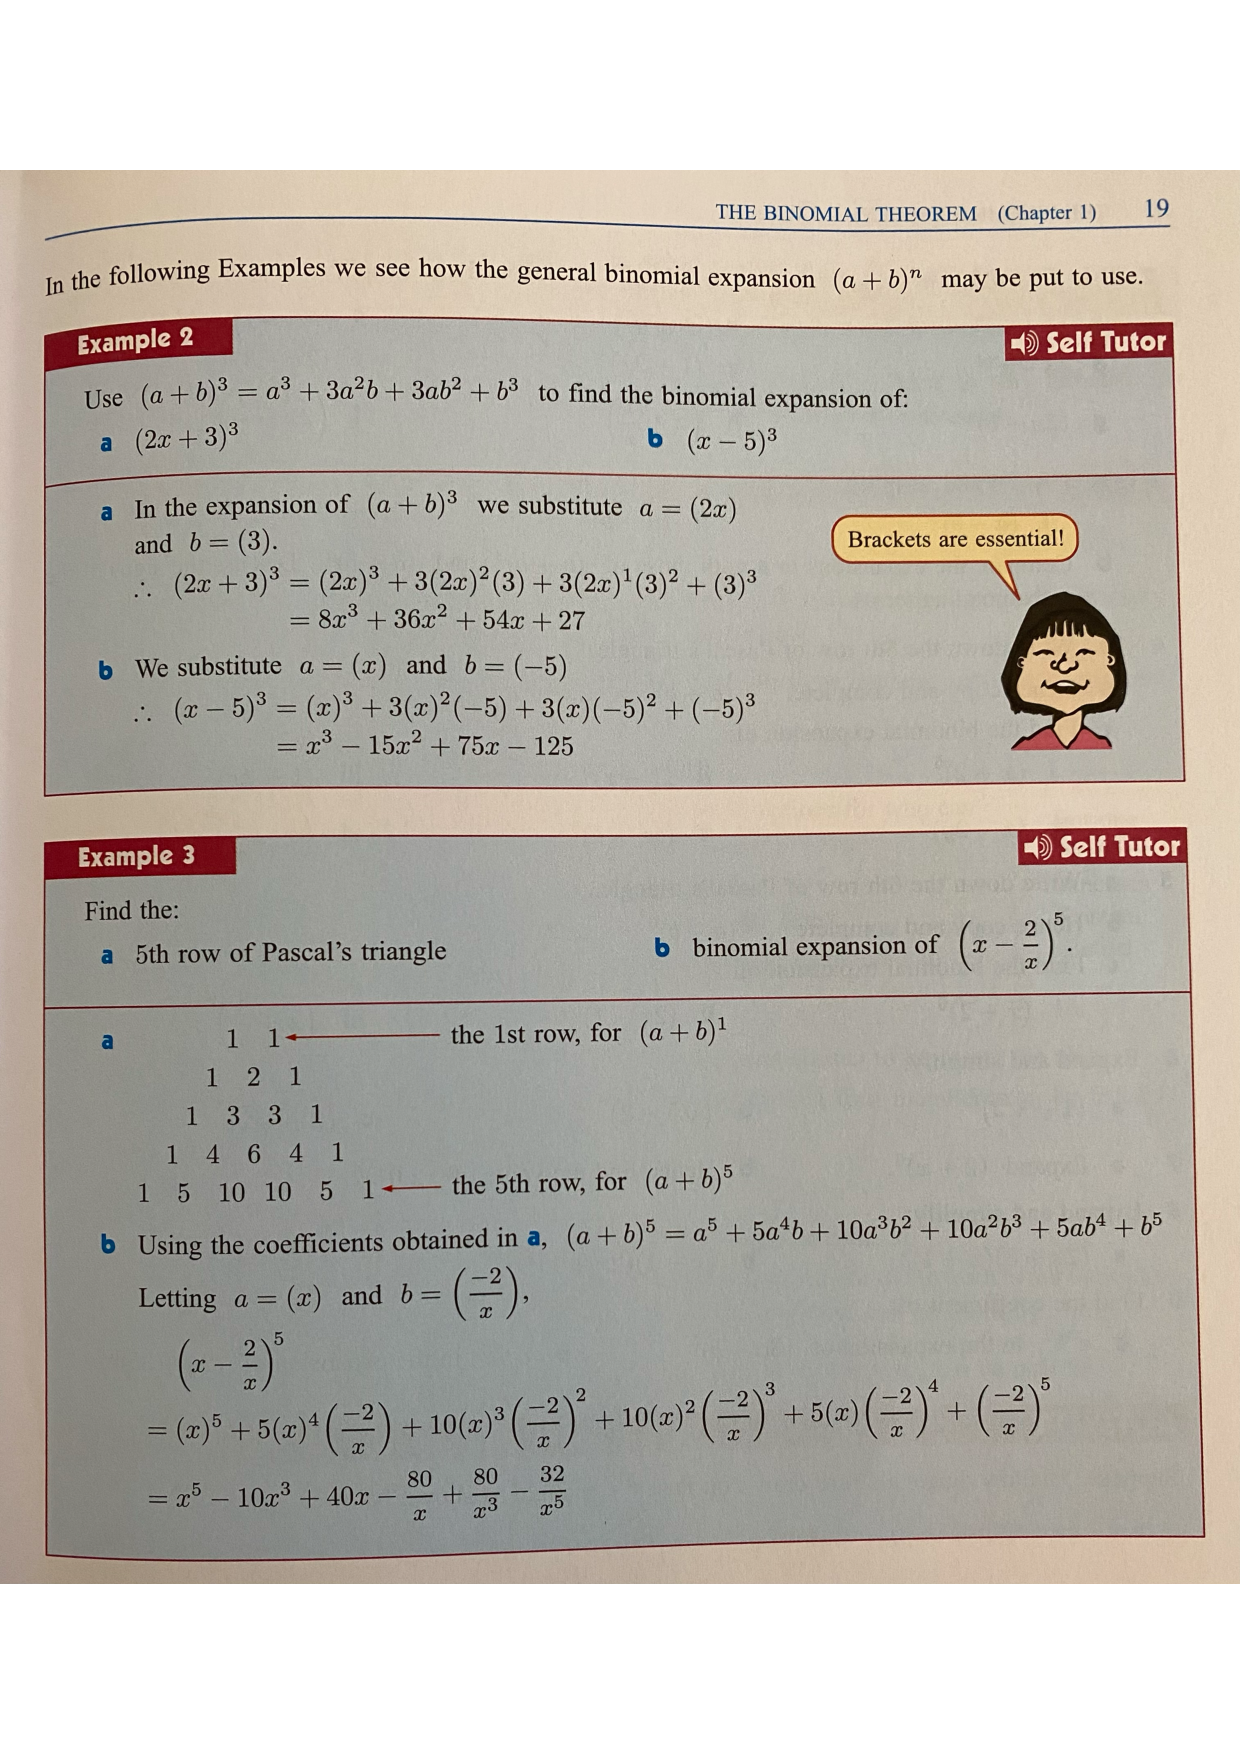
\includegraphics[width=16cm]{BinomialExpansionExampleTextB.pdf}
\end{figure}
\newpage
\subsection{Ex 1B}
\newpage
\includepdf[pages={1-},scale=0.9]{BinomialExpansionsQuestions.pdf} 
\newpage
\section{Binomial Theorem}
Counting:\\
\begin{enumerate}[leftmargin=0.5cm]
	\item How many ways can the letters AB be organised?:\\\LineControl{1}{1cm}{17cm}
	\item How many ways can the letters ABC be organised?:\\\LineControl{1}{1cm}{17cm}
	\item How many ways can the letters ABCDE be organised?:\\\LineControl{1}{1cm}{17cm}
\end{enumerate}
\begin{enumerate}[leftmargin=0.5cm]
	\item How many ways can the letters AABBB be organised?:\\\LineControl{1}{1cm}{17cm}
	\item How many ways can the letters ABBBB be organised?:\\\LineControl{1}{1cm}{17cm}
\end{enumerate}
If we consider the expansion of $(a+b)^5$\\
There will be:
\begin{itemize}[itemsep=0.5cm]
\item  \rule{4cm}{0.1pt} combinations of  $aaaaa$ ($a^5$)
\item \rule{4cm}{0.1pt} combinations of  $aaaab$ ($a^4b$)
\item  \rule{4cm}{0.1pt} combinations of  $aaabb$ ($a^3b^2$)
\item  \rule{4cm}{0.1pt} combinations of  $aabbb$ ($a^2b^3$)
\item  \rule{4cm}{0.1pt} combinations of  $abbbb$ ($ab^4$)
\item  \rule{4cm}{0.1pt} combinations of  $bbbbb$ ($b^5$)
\end{itemize}
\newpage
We can see for a string of length $\mathbf{n}$ using only the letters $a$ and $b$, the number of possible combinations of a string containing $\mathbf{r}$ occurrances of a ( and consequently $\mathbf{n-r}$ occurrances of $b$ )  will be
$$ \displaystyle  \binom{n}{k} = \frac{n!}{k!(n-k)!} $$
This is a different way of explaining from the book, but the result is the same.\\
We can now state the binomial theorem that:
\begin{alignat*}{2}
		(a+b)^n&=\binom{n}{0} a^nb^0 + \binom{n}{1}a^{n-1}b^1 + ...+\binom{n}{r} a^{n-r}b^{r} +... + \binom{n}{n-1} a^1b^{n-1} +\binom{n}{n} a^0b^{n} &&\\\\
		(a+b)^n&= a^n + \binom{n}{1}a^{n-1}b+ ...+\binom{n}{r} a^{n-r}b^{r} +... + \binom{n}{n-1} ab^{n-1} + b^{n}&& \\\\
		(a+b)^n&= \sum_{r=0}^{n}~ \binom{n}{r} a^{n-r}b^r \text{~~~~~~~~~Binomial Theorem}& &
\end{alignat*}
The \textbf{general term} or $(r+1)^{th}$ term is:
$$T_{k+1} = \binom{n}{r} a^{n-r}b^r $$
So the first term is: ~~~$\displaystyle T_1 = T_{0+1} =  \binom{n}{0}a^{n-0}b^0 = a^n$



\subsection{Ex 1C}
\newpage
\includepdf[pages={1-},scale=0.9]{BinomialTheoremQuestions.pdf} 
\newpage
\section{Review Sets}
\newpage
\section{Summary formulae}
\def\arraystretch{3}
\setlength\tabcolsep{1cm}
\newcommand{\pad}{0.2cm}
\begin{center}
	\begin{tabular}{| c | M |} \hline
		Binomial Theorem   & \displaystyle (a+b)^n= \sum_{k=0}^{n}~ \binom{n}{k} a^{n-k}b^k \\ [\pad] \hline
		Combination Definition & \displaystyle  \binom{n}{k} = \frac{n!}{k!(n-k)!} \\ [\pad] \hline
		First and Last & \displaystyle  \binom{n}{0} =\binom{n}{n} = 1\\ [\pad] \hline
		A term in the expansion  &\displaystyle  T_{k+1} = \binom{n}{k} a^{n-k}b^k \\ [\pad] \hline
		Pascal's identity  &\displaystyle \binom{n}{k} = \binom{n-1}{k-1} + \binom{n-1}{k} \\ [\pad] \hline
		Symmetry &\displaystyle  \binom{n}{k} = \binom{n}{n-k} \\ [\pad] \hline
	\end{tabular}
\end{center}
\section{Extra questions}
\begin{enumerate}
	\item In the expansion of $(a–3b)^n$, the sum of 9th and 10th term is zero. \\
	Find the value of  $\frac{a}{b}$ in terms of $n$ in terms of  n
	\item  If the coefficient of 5th, 6th and 7th terms in the expansion of  $(1+x)^n$ are in arithmetic sequence, then find the value(s) of n
	\item If $x_n - y_n\sqrt{2} = (1- \sqrt{2})^n$, then show that $x_n^{~2} - 2y_n^{~2} = (-1)^n$
	\item Find the first three terms in the expansion, in ascending powers of $x$, of $(1–2x)^5$
	\item Given that the coefficient of $x^2$ in the expansion of $(1+ax+2x^2)(1–2x)^5$ is 12, find the value of the constant $a$.
	\item ~
	\begin{enumerate}
		\item Use the binomial theorem to expand  $(a+\sqrt{b})^4$
		\item  Hence, deduce an expression in terms of  $a$ and  $b$ for $(a+\sqrt{b})^4 + (a-\sqrt{b})^4$
	\end{enumerate}
	\item ~
	\begin{enumerate}
		\item Write down and simplify the general term in the binomial expansion of $\displaystyle (2x^2– \frac{d}{x^3})^7$ , where  d is a constant
		\item Given that the coefficient of $\displaystyle \frac{1}{x}$ is $-70,000$ find the value of $d$
	\end{enumerate}
	
\end{enumerate}

\newpage
\includepdf[pages={1-},scale=0.9]{BinomialQsExtra.pdf} 
\newpage

\end{document}